\chapter{RoBee}\label{chap:robee}
RoBee è un robot umanoide made in Italy, sviluppato e costruito a Besana Brianza dall'azienda Oversonic Robotics presso la quale ho svolto la mia esperienza di tirocinio.\\\\
È un robot la cui altezza varia dai 135 ai 200 cm in funzione della configurazione dei giunti delle gambe, ha 39 gradi di libertà e un ingombro in pianta di 65 cm quadrati. L'estensione del braccio può arrivare fino a 80 cm e può navigare fino a una velocità di 1.2 m/s. È dotato di certificazioni industriali e di sicurezza.
\begin{figure}[H]
  \centering
  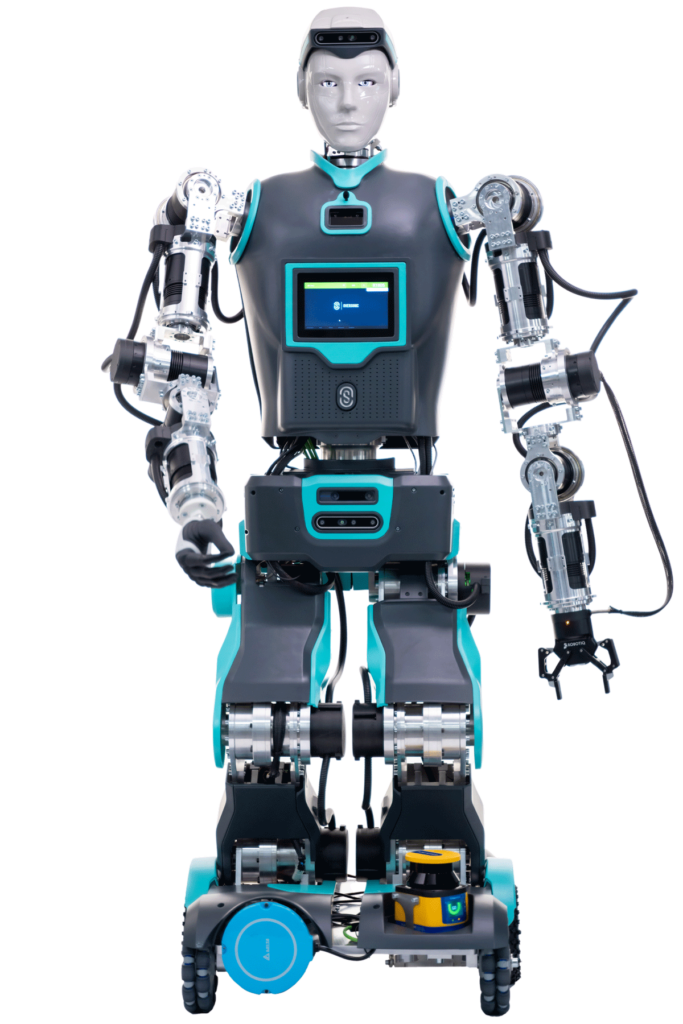
\includegraphics[width=0.45\textwidth]{robee_18.png}
  \caption{Robee in versione 18}
\end{figure}
\section{Architettura Cloud Native}
L'architettura di RoBee è basata su microservizi la cui orchestrazione è gestita da Kubernetes. Ci sono due tipologie di container:
\begin{itemize}
  \item Moduli: pod che vengono eseguiti localmente su ogni Robot e gestiscono le varie funzionalità di base del robot, come la navigazione, la gestione dei giunti, dello streaming delle camera e così via. La gestione dei pod sulle macchine locali è gestita da \gls{kubeedge}
  \item Servizi: pod che vengono eseguiti sul cloud e gestiscono funzionalità piú generali e che non sono strettamente legate al singolo robot. Un esempio di servizio è \textit{scene perception}, il modulo sviluppato durante il tirocinio il cui funzionamento è descritto in questa tesi.
\end{itemize}
RoBee è dotato di innumerevoli moduli e servizi ma in questa sezione verrano illustrati brevemente solo quelli che sono strettamente legati al funzionamento di \textit{scene perception} e di questa tesi.
\section{Dashboard and Console}
Dashboard e Console sono due servizi utilizzati per la gestione dei robot, delle mappe, delle missioni e tante altre funzionalità.\\
Entrambe le applicazioni web sono state sviluppate con lo stack Python, Tornado, Turbo e Stimulus JS.
\subsection{Dashboard}
La dashboard è lo strumento principale per gli sviluppatori e gli utentidi Oversonic per la gestione dei moduli e dei servizi. Attraverso la dashboard è possibile:
\begin{itemize}
  \item Aggiornare i Moduli e i Servizi;
  \item Monitorare i log dei Servizi;
  \item Disabilitare e abilitare i Moduli per ogni robot;
  \item Disabilitare e abilitare i Servizi e scegliere per ogni robot verso quale servizio "puntare": è infatti possibile per debug far puntare un robot a un servizio diverso in esecuzione sui PC degli sviluppatori piuttosto che a quello di produzione;
  \item Modificare le configurazione dei Robot, Moduli o Servizi.
\end{itemize}
\subsection{Console}
La console è lo strumento principale per gli utenti finali per la gestione dei robot e di tutto ciò che lo riguarda. Attraverso la console è possibile:
\begin{itemize}
  \item Monitorare la telemetria dei robot in tempo reale;
  \item Programmare missioni attraverso un tool visuale;
  \item Visualizzare la mappa e modificarne i layer semantici, tra cui quello delle stanze oggetto del capitolo \ref{chap:riconoscimento_stanze};
  \item Impostare goal nella mappa;
  \item Creare, Modificare o Eliminare le mappe;
  \item Muovere manualmente il robot;
  \item Visualizzare il feed proveniente dalle telecamere.
\end{itemize}

\section{Mappe, navigazione e LiDaR}
Il sistema di navigazione di RoBee è basato su ruote omnidirezionali la cui gestione avviene attraverso navigation module. Attraverso l'utilizzo dei LiDar è possibile mappare l'ambienete, localizzarsi e prevenire movimenti che potrebbero causare danni al robot o all'ambiente.\\
Il modulo è il responsabile della creazione della grid map di occupazione: riceve i dati, costruisce la mappa ed effettua una chiamata http ad API Service per effettuare il riconoscimento delle stanze e salvarla sul database.

\section{Giunti e controllo}
La gestione dei giunti è affidata a Joints Module, che si occupa di tener traccia dello stato, posizione e rotazione, di ogni giunto del robot nel tempo. Inoltre
gestisce l'albero delle TF: soddisfa le richieste degli altri moduli, tramite MQTT, per ottenere la matrice di trasformazione tra due sistemi di riferimento.

\section{Camere e point cloud}
Robee è dotato di 4 telecamere base: \textit{head}, \textit{navigation}, \textit{back} e \textit{face recognition}. In aggiunta a queste, è possibile montare telecamera sul braccio apposite per gli end effectors.\\
La gestione delle camere è affidata a streaming module che si occupa di leggere i frame dalle telecamere e streammarli su Redis per renderli disponibili ai moduli o servizi che ne fanno richiesta. Per esempio, scene perception si interfaccia al pod Redis eseguito on edge su un robot per poter leggere i frame provenienti dalla camera selezionata per fare inferenza. \\
In base alla tipologia di modello di telecamera, è possibile ottenere anche la point cloud, ovvero una rappresentazione tridimensionale dell'ambiente circostante il robot.

